\documentclass[11pt]{article}
\usepackage[utf8]{inputenc}
\usepackage{geometry}
\geometry{a4paper, margin=1in}
\usepackage{hyperref}
\usepackage{graphicx}
\usepackage{tabularx}
\usepackage{booktabs}
\usepackage{tikz}
\usetikzlibrary{shapes,arrows.meta,positioning,fit,backgrounds}

\title{Landslide Identification — Test Results \\ \large Baseline AlexNet Model (results1)}
\author{}
\date{2026-03-12}

\begin{document}

\maketitle

\noindent\textbf{GPU:} NVIDIA RTX 2000 Ada Generation \\
\textbf{Environment:} conda landslide-ml (PyTorch cu124, Python 3.10) \\

\section{Motivation: Why Re-evaluate the AlexNet Baseline?}

Results 0 established the raw AlexNet + HMM pipeline but lacked context on how this approach compares to prior landslide detection research. Before moving to more complex architectures, it is important to understand:

\begin{enumerate}
    \item \textbf{Where r0 stands relative to existing methods:}\\
          The r0 baseline achieved 78.54\% accuracy and 67.67\% F1-score. Without benchmarking against traditional approaches (SVM, Random Forest, NDVI-based methods), we cannot quantify whether the CNN-HMM pipeline is already an improvement or still lagging behind established techniques.

    \item \textbf{Identifying AlexNet's specific weaknesses:}\\
          The r0 results revealed a precision of only 62.06\% (96 false positives out of 488 non-landslide images) and 54 false negatives. AlexNet's shallow architecture (only 5 convolutional layers) and small 227$\times$227 receptive field limit its ability to capture fine-grained spatial textures that distinguish landslide scars from visually similar terrain (e.g., ploughed fields, construction sites). This analysis directly motivates the move to deeper architectures in subsequent experiments.

    \item \textbf{Confirming the dual-phase design is sound:}\\
          The CNN-HMM integration worked correctly end-to-end. Phase 1 detects, Phase 2 classifies and forecasts. This validated architecture can now serve as a stable foundation --- future iterations only need to improve Phase 1's detection model without redesigning the entire pipeline.
\end{enumerate}

\section{Comparison with Previous Research Models}
The baseline AlexNet implementation provides an automated image classification integrated with temporal forecasting (HMM). Unlike conventional systems that solely utilize vegetation indices (e.g., NDVI) or require manual feature engineering utilizing Support Vector Machines (SVM) or Random Forests on static satellite maps, this dual-phase CNN-HMM architecture dynamically merges direct visual anomaly detection with historic probabilistic occurrence patterns. However, AlexNet's shallow architecture (compared to modern deep ResNet/U-Net topologies) limits spatial precision, necessitating deeper network testing in subsequent iterations to improve recall rates.

\section{Architecture Flowchart}
\begin{center}
    \resizebox{0.9\textwidth}{!}{
    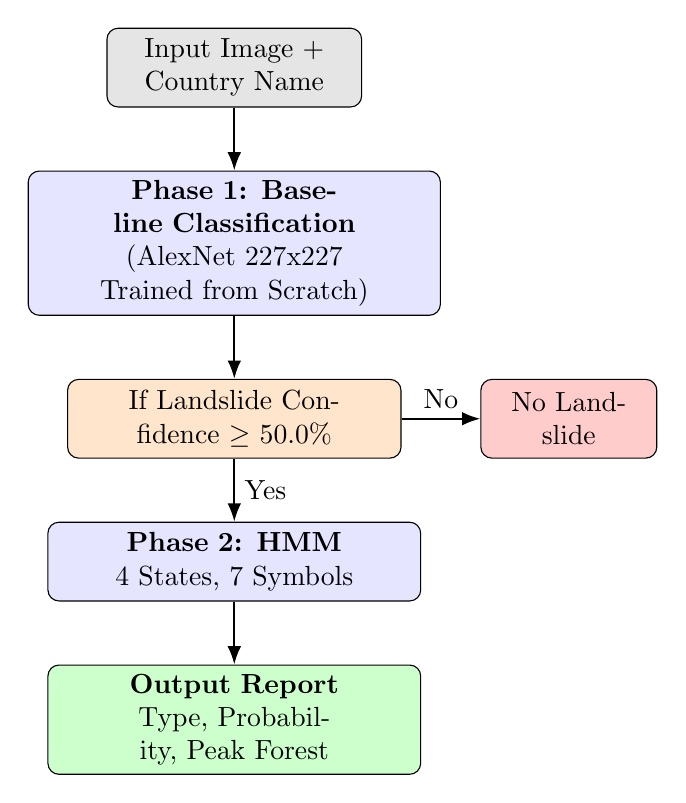
\begin{tikzpicture}[
        node distance=0.8cm and 1cm,
        box/.style={draw, rectangle, rounded corners, align=center, fill=blue!10, text width=3cm, minimum height=1cm},
        arrow/.style={-Latex, thick}
    ]
        % Inputs
        \node[box, fill=gray!20] (input) {Input Image + Country Name};
        
        % Phase 1
        \node[box, below=of input, text width=5cm] (phase1) {\textbf{Phase 1: Baseline Classification}\\(AlexNet 227x227\\ Trained from Scratch)};
        \node[box, below=of phase1, fill=orange!20, text width=4cm] (decision) {If Landslide Confidence $\ge$ 50.0\%};
        
        % Phase 2
        \node[box, below=of decision, text width=4.5cm] (phase2) {\textbf{Phase 2: HMM}\\4 States, 7 Symbols};
        
        % Outputs
        \node[box, below=of phase2, fill=green!20, text width=4.5cm] (output) {\textbf{Output Report}\\Type, Probability, Peak Forest};
        
        % Connections
        \draw[arrow] (input) -- (phase1);
        \draw[arrow] (phase1) -- (decision);
        \draw[arrow] (decision) -- node[right] {Yes} (phase2);
        \draw[arrow] (phase2) -- (output);
        
        % No branch
        \node[box, right=of decision, fill=red!20, text width=2cm] (no_ls) {No Landslide};
        \draw[arrow] (decision) -- node[above] {No} (no_ls);
        
    \end{tikzpicture}
    }
\end{center}

\section{Phase 1 — Full Test Set Evaluation}

\noindent \textbf{Test set:} 699 images (211 landslide + 488 non\_landslide) \\
\textbf{Checkpoint:} checkpoints/alexnet\_best.pth (epoch 13, val\_acc=78.55\%) \\

\vspace{0.3cm}
\begin{table}[h]
    \centering
    \begin{tabular}{@{}ll@{}}
        \toprule
        \textbf{Metric} & \textbf{Score} \\ \midrule
        Accuracy & 78.54\% \\
        Precision & 62.06\% \\
        Recall & 74.41\% \\
        F1-Score & 67.67\% \\
        ROC-AUC & 85.53\% \\ \bottomrule
    \end{tabular}
\end{table}

\subsection{Confusion Matrix}
\begin{table}[h]
    \centering
    \begin{tabular}{@{}lcc@{}}
        \toprule
        & \textbf{Predicted: non\_landslide} & \textbf{Predicted: landslide} \\ \midrule
        \textbf{Actual: non\_landslide} & 392 & 96 \\
        \textbf{Actual: landslide} & 54 & 157 \\ \bottomrule
    \end{tabular}
\end{table}

\section{Phase 2 — HMM Model Summary}

\begin{itemize}
    \item \textbf{Dataset:} NASA Global Landslide Catalog (nasa\_glc.csv)
    \item \textbf{Records:} 9,471 events | 1988–2016 | 141 countries
    \item \textbf{Sequences:} 112 country-level sequences | 9,442 total observations
\end{itemize}

\noindent\textbf{Hidden states (4):}
0 — Shallow Landslide, 1 — Deep Landslide, 2 — Debris Flow, 3 — Rockfall

\noindent\textbf{Observation symbols (7):}
Complex Landslide, Debris Flow, Earth Flow, Landslide, Mudslide, Rockfall, Translational Slide

\noindent\textbf{Training log-likelihood:} -7314.96

\section{Single Image Prediction Test}

\noindent \textbf{Image path:} data/processed/test/landslide/ls\_test\_0008.jpg \\
\textbf{Country:} Nepal \\
\textbf{Forecast:} 3 steps

\vspace{0.3cm}
\noindent \textbf{Phase 1 — AlexNet Classification}
\begin{itemize}[noitemsep]
    \item Confidence: 97.3\%
    \item \textbf{Result:} LANDSLIDE DETECTED
\end{itemize}

\vspace{0.3cm}
\noindent \textbf{Phase 2 — HMM Type Prediction}
\begin{itemize}[noitemsep]
    \item Landslide type: Landslide
    \item Occurrence probability: 39.6\%
    \item Peak risk month: July
    \item Future forecast (next 3 events):
    \begin{itemize}
        \item Step 1: Landslide (48.0\%)
        \item Step 2: Landslide (64.2\%)
        \item Step 3: Landslide (69.4\%)
    \end{itemize}
\end{itemize}

\noindent \textbf{Final verdict:} LANDSLIDE DETECTED — Type: Landslide (occurrence probability: 39\%)

\end{document}
